\documentclass[twoside]{book}

% Packages required by doxygen
\usepackage{fixltx2e}
\usepackage{calc}
\usepackage{doxygen}
\usepackage[export]{adjustbox} % also loads graphicx
\usepackage{graphicx}
\usepackage[utf8]{inputenc}
\usepackage{makeidx}
\usepackage{multicol}
\usepackage{multirow}
\PassOptionsToPackage{warn}{textcomp}
\usepackage{textcomp}
\usepackage[nointegrals]{wasysym}
\usepackage[table]{xcolor}

% Font selection
\usepackage[T1]{fontenc}
\usepackage[scaled=.90]{helvet}
\usepackage{courier}
\usepackage{amssymb}
\usepackage{sectsty}
\renewcommand{\familydefault}{\sfdefault}
\allsectionsfont{%
  \fontseries{bc}\selectfont%
  \color{darkgray}%
}
\renewcommand{\DoxyLabelFont}{%
  \fontseries{bc}\selectfont%
  \color{darkgray}%
}
\newcommand{\+}{\discretionary{\mbox{\scriptsize$\hookleftarrow$}}{}{}}

% Page & text layout
\usepackage{geometry}
\geometry{%
  a4paper,%
  top=2.5cm,%
  bottom=2.5cm,%
  left=2.5cm,%
  right=2.5cm%
}
\tolerance=750
\hfuzz=15pt
\hbadness=750
\setlength{\emergencystretch}{15pt}
\setlength{\parindent}{0cm}
\setlength{\parskip}{3ex plus 2ex minus 2ex}
\makeatletter
\renewcommand{\paragraph}{%
  \@startsection{paragraph}{4}{0ex}{-1.0ex}{1.0ex}{%
    \normalfont\normalsize\bfseries\SS@parafont%
  }%
}
\renewcommand{\subparagraph}{%
  \@startsection{subparagraph}{5}{0ex}{-1.0ex}{1.0ex}{%
    \normalfont\normalsize\bfseries\SS@subparafont%
  }%
}
\makeatother

% Headers & footers
\usepackage{fancyhdr}
\pagestyle{fancyplain}
\fancyhead[LE]{\fancyplain{}{\bfseries\thepage}}
\fancyhead[CE]{\fancyplain{}{}}
\fancyhead[RE]{\fancyplain{}{\bfseries\leftmark}}
\fancyhead[LO]{\fancyplain{}{\bfseries\rightmark}}
\fancyhead[CO]{\fancyplain{}{}}
\fancyhead[RO]{\fancyplain{}{\bfseries\thepage}}
\fancyfoot[LE]{\fancyplain{}{}}
\fancyfoot[CE]{\fancyplain{}{}}
\fancyfoot[RE]{\fancyplain{}{\bfseries\scriptsize Generated by Doxygen }}
\fancyfoot[LO]{\fancyplain{}{\bfseries\scriptsize Generated by Doxygen }}
\fancyfoot[CO]{\fancyplain{}{}}
\fancyfoot[RO]{\fancyplain{}{}}
\renewcommand{\footrulewidth}{0.4pt}
\renewcommand{\chaptermark}[1]{%
  \markboth{#1}{}%
}
\renewcommand{\sectionmark}[1]{%
  \markright{\thesection\ #1}%
}

% Indices & bibliography
\usepackage{natbib}
\usepackage[titles]{tocloft}
\setcounter{tocdepth}{3}
\setcounter{secnumdepth}{5}
\makeindex

% Hyperlinks (required, but should be loaded last)
\usepackage{ifpdf}
\ifpdf
  \usepackage[pdftex,pagebackref=true]{hyperref}
\else
  \usepackage[ps2pdf,pagebackref=true]{hyperref}
\fi
\hypersetup{%
  colorlinks=true,%
  linkcolor=blue,%
  citecolor=blue,%
  unicode%
}

% Custom commands
\newcommand{\clearemptydoublepage}{%
  \newpage{\pagestyle{empty}\cleardoublepage}%
}

\usepackage{caption}
\captionsetup{labelsep=space,justification=centering,font={bf},singlelinecheck=off,skip=4pt,position=top}

%===== C O N T E N T S =====

\begin{document}

% Titlepage & ToC
\hypersetup{pageanchor=false,
             bookmarksnumbered=true,
             pdfencoding=unicode
            }
\pagenumbering{alph}
\begin{titlepage}
\vspace*{7cm}
\begin{center}%
{\Large Key Listener Using Search History \\[1ex]\large 1.\+0 }\\
\vspace*{1cm}
{\large Generated by Doxygen 1.8.13}\\
\end{center}
\end{titlepage}
\clearemptydoublepage
\pagenumbering{roman}
\tableofcontents
\clearemptydoublepage
\pagenumbering{arabic}
\hypersetup{pageanchor=true}

%--- Begin generated contents ---
\chapter{Namespace Index}
\section{Namespace List}
Here is a list of all namespaces with brief descriptions\+:\begin{DoxyCompactList}
\item\contentsline{section}{\hyperlink{namespacekeylistener}{keylistener} }{\pageref{namespacekeylistener}}{}
\end{DoxyCompactList}

\chapter{Hierarchical Index}
\section{Class Hierarchy}
This inheritance list is sorted roughly, but not completely, alphabetically\+:\begin{DoxyCompactList}
\item \contentsline{section}{keylistener.\+File\+History}{\pageref{classkeylistener_1_1_file_history}}{}
\item J\+Frame\begin{DoxyCompactList}
\item \contentsline{section}{keylistener.\+Key\+G\+UI}{\pageref{classkeylistener_1_1_key_g_u_i}}{}
\end{DoxyCompactList}
\item \contentsline{section}{keylistener.\+Read\+File}{\pageref{classkeylistener_1_1_read_file}}{}
\item \contentsline{section}{keylistener.\+Search}{\pageref{classkeylistener_1_1_search}}{}
\end{DoxyCompactList}

\chapter{Class Index}
\section{Class List}
Here are the classes, structs, unions and interfaces with brief descriptions\+:\begin{DoxyCompactList}
\item\contentsline{section}{\hyperlink{classkeylistener_1_1_key_g_u_i_1_1_file_action}{keylistener.\+Key\+G\+U\+I.\+File\+Action} }{\pageref{classkeylistener_1_1_key_g_u_i_1_1_file_action}}{}
\item\contentsline{section}{\hyperlink{classkeylistener_1_1_file_history}{keylistener.\+File\+History} }{\pageref{classkeylistener_1_1_file_history}}{}
\item\contentsline{section}{\hyperlink{classkeylistener_1_1_key_g_u_i_1_1_history_action}{keylistener.\+Key\+G\+U\+I.\+History\+Action} }{\pageref{classkeylistener_1_1_key_g_u_i_1_1_history_action}}{}
\item\contentsline{section}{\hyperlink{classkeylistener_1_1_key_g_u_i}{keylistener.\+Key\+G\+UI} }{\pageref{classkeylistener_1_1_key_g_u_i}}{}
\item\contentsline{section}{\hyperlink{classkeylistener_1_1_read_file}{keylistener.\+Read\+File} }{\pageref{classkeylistener_1_1_read_file}}{}
\item\contentsline{section}{\hyperlink{classkeylistener_1_1_search}{keylistener.\+Search} }{\pageref{classkeylistener_1_1_search}}{}
\item\contentsline{section}{\hyperlink{classkeylistener_1_1_key_g_u_i_1_1_search_action}{keylistener.\+Key\+G\+U\+I.\+Search\+Action} }{\pageref{classkeylistener_1_1_key_g_u_i_1_1_search_action}}{}
\end{DoxyCompactList}

\chapter{File Index}
\section{File List}
Here is a list of all files with brief descriptions\+:\begin{DoxyCompactList}
\item\contentsline{section}{src/keylistener/\hyperlink{_file_history_8java}{File\+History.\+java} }{\pageref{_file_history_8java}}{}
\item\contentsline{section}{src/keylistener/\hyperlink{_key_g_u_i_8java}{Key\+G\+U\+I.\+java} }{\pageref{_key_g_u_i_8java}}{}
\item\contentsline{section}{src/keylistener/\hyperlink{_read_file_8java}{Read\+File.\+java} }{\pageref{_read_file_8java}}{}
\item\contentsline{section}{src/keylistener/\hyperlink{_search_8java}{Search.\+java} }{\pageref{_search_8java}}{}
\end{DoxyCompactList}

\chapter{Namespace Documentation}
\hypertarget{namespacekeylistener}{}\section{Package keylistener}
\label{namespacekeylistener}\index{keylistener@{keylistener}}
\subsection*{Classes}
\begin{DoxyCompactItemize}
\item 
class \hyperlink{classkeylistener_1_1_file_history}{File\+History}
\item 
class \hyperlink{classkeylistener_1_1_key_g_u_i}{Key\+G\+UI}
\item 
class \hyperlink{classkeylistener_1_1_read_file}{Read\+File}
\item 
class \hyperlink{classkeylistener_1_1_search}{Search}
\end{DoxyCompactItemize}

\chapter{Class Documentation}
\hypertarget{classkeylistener_1_1_file_history}{}\section{keylistener.\+File\+History Class Reference}
\label{classkeylistener_1_1_file_history}\index{keylistener.\+File\+History@{keylistener.\+File\+History}}
\subsection*{Public Member Functions}
\begin{DoxyCompactItemize}
\item 
\hyperlink{classkeylistener_1_1_file_history_a22f91ebaebdafb0076fc7ff28c3f1993}{File\+History} ()
\item 
\hyperlink{classkeylistener_1_1_file_history_a31c068625f0fdac8966c4ce76bde8a86}{File\+History} (String file, String keyword, String\mbox{[}$\,$\mbox{]} lst\+Result, String date)
\item 
String \hyperlink{classkeylistener_1_1_file_history_a3566b314572e386b54c140ab4936590b}{get\+File\+Name} ()
\item 
String \hyperlink{classkeylistener_1_1_file_history_a33c2c0514f7fc3614f428504dd74276d}{get\+Input\+Search} ()
\item 
String \mbox{[}$\,$\mbox{]} \hyperlink{classkeylistener_1_1_file_history_a25a150f439e4577a25b29fbf9f86f9b7}{get\+Results} ()
\item 
\hyperlink{classkeylistener_1_1_file_history}{File\+History} \hyperlink{classkeylistener_1_1_file_history_ae89875744c0f07e59f8e2087c985901c}{get\+Previous} ()
\item 
\hyperlink{classkeylistener_1_1_file_history}{File\+History} \hyperlink{classkeylistener_1_1_file_history_a6a27d9d0c37dd7cc422bd6bd6ca709be}{get\+Next} ()
\item 
String \hyperlink{classkeylistener_1_1_file_history_a72fefe056f783ec704374f9c14dda0a5}{get\+Date} ()
\item 
void \hyperlink{classkeylistener_1_1_file_history_a721185583f76cb336eb489e0124a8be8}{set\+File\+Name} (String file)
\item 
void \hyperlink{classkeylistener_1_1_file_history_acaf8a8e1dc879a8ef64e0940ab791bc7}{set\+Input\+Search} (String input)
\item 
void \hyperlink{classkeylistener_1_1_file_history_a7e8911bcdd6a7483ba7e317692af39c9}{set\+Results} (String\mbox{[}$\,$\mbox{]} s\+Result)
\item 
void \hyperlink{classkeylistener_1_1_file_history_ab3c4c436053b547e327b04b812a9870c}{set\+Previous} (\hyperlink{classkeylistener_1_1_file_history}{File\+History} before)
\item 
void \hyperlink{classkeylistener_1_1_file_history_a8e5dff723fb93991057375f579486eae}{set\+Next} (\hyperlink{classkeylistener_1_1_file_history}{File\+History} after)
\item 
void \hyperlink{classkeylistener_1_1_file_history_a1de701cd56aac77075457d16c411be74}{set\+Date} (String date)
\end{DoxyCompactItemize}
\subsection*{Private Attributes}
\begin{DoxyCompactItemize}
\item 
\hyperlink{classkeylistener_1_1_file_history}{File\+History} \hyperlink{classkeylistener_1_1_file_history_ab08fec8e2a293a9000087d18e1454c44}{previous}
\item 
\hyperlink{classkeylistener_1_1_file_history}{File\+History} \hyperlink{classkeylistener_1_1_file_history_aa9571ba3eabdcc6b9e7d152a0a7537ee}{next}
\item 
String \hyperlink{classkeylistener_1_1_file_history_aa039d04ae73d6098a0d63f42dcf7a953}{file\+Name}
\item 
String \hyperlink{classkeylistener_1_1_file_history_a6370f7f80f43860c1da4962b9e0a3f01}{search}
\item 
String \mbox{[}$\,$\mbox{]} \hyperlink{classkeylistener_1_1_file_history_a665862b474b78805e841aaf23ab1123c}{results}
\item 
String \hyperlink{classkeylistener_1_1_file_history_aa05796c787baef3237827630d3284496}{search\+Date}
\end{DoxyCompactItemize}


\subsection{Detailed Description}
\hyperlink{classkeylistener_1_1_file_history}{File\+History} --- this class contains the search history from inside of the file. It used a double linked list to check the previous and next search items in the history. \begin{DoxyAuthor}{Author}
Van Do 
\end{DoxyAuthor}


\subsection{Constructor \& Destructor Documentation}
\mbox{\Hypertarget{classkeylistener_1_1_file_history_a22f91ebaebdafb0076fc7ff28c3f1993}\label{classkeylistener_1_1_file_history_a22f91ebaebdafb0076fc7ff28c3f1993}} 
\index{keylistener\+::\+File\+History@{keylistener\+::\+File\+History}!File\+History@{File\+History}}
\index{File\+History@{File\+History}!keylistener\+::\+File\+History@{keylistener\+::\+File\+History}}
\subsubsection{\texorpdfstring{File\+History()}{FileHistory()}\hspace{0.1cm}{\footnotesize\ttfamily [1/2]}}
{\footnotesize\ttfamily keylistener.\+File\+History.\+File\+History (\begin{DoxyParamCaption}{ }\end{DoxyParamCaption})\hspace{0.3cm}{\ttfamily [inline]}}

Null class constructor to access methods. \mbox{\Hypertarget{classkeylistener_1_1_file_history_a31c068625f0fdac8966c4ce76bde8a86}\label{classkeylistener_1_1_file_history_a31c068625f0fdac8966c4ce76bde8a86}} 
\index{keylistener\+::\+File\+History@{keylistener\+::\+File\+History}!File\+History@{File\+History}}
\index{File\+History@{File\+History}!keylistener\+::\+File\+History@{keylistener\+::\+File\+History}}
\subsubsection{\texorpdfstring{File\+History()}{FileHistory()}\hspace{0.1cm}{\footnotesize\ttfamily [2/2]}}
{\footnotesize\ttfamily keylistener.\+File\+History.\+File\+History (\begin{DoxyParamCaption}\item[{String}]{file,  }\item[{String}]{keyword,  }\item[{String \mbox{[}$\,$\mbox{]}}]{lst\+Result,  }\item[{String}]{date }\end{DoxyParamCaption})\hspace{0.3cm}{\ttfamily [inline]}}

Parameterized constructor to store object\textquotesingle{}s file history data 
\begin{DoxyParams}{Parameters}
{\em file} & -\/ the name of the file. See \hyperlink{classkeylistener_1_1_file_history_aa039d04ae73d6098a0d63f42dcf7a953}{file\+Name}. \\
\hline
{\em keyword} & -\/ the user input for searching the line. See \hyperlink{classkeylistener_1_1_file_history_a6370f7f80f43860c1da4962b9e0a3f01}{search}. \\
\hline
{\em lst\+Result} & -\/ the results that contain compared lines. See \hyperlink{classkeylistener_1_1_file_history_a665862b474b78805e841aaf23ab1123c}{results}. \\
\hline
{\em date} & -\/ the search date that have been found. See \hyperlink{classkeylistener_1_1_file_history_aa05796c787baef3237827630d3284496}{search\+Date}. \\
\hline
\end{DoxyParams}


\subsection{Member Function Documentation}
\mbox{\Hypertarget{classkeylistener_1_1_file_history_a72fefe056f783ec704374f9c14dda0a5}\label{classkeylistener_1_1_file_history_a72fefe056f783ec704374f9c14dda0a5}} 
\index{keylistener\+::\+File\+History@{keylistener\+::\+File\+History}!get\+Date@{get\+Date}}
\index{get\+Date@{get\+Date}!keylistener\+::\+File\+History@{keylistener\+::\+File\+History}}
\subsubsection{\texorpdfstring{get\+Date()}{getDate()}}
{\footnotesize\ttfamily String keylistener.\+File\+History.\+get\+Date (\begin{DoxyParamCaption}{ }\end{DoxyParamCaption})\hspace{0.3cm}{\ttfamily [inline]}}

Return the search date of this search item. See \hyperlink{classkeylistener_1_1_file_history_aa05796c787baef3237827630d3284496}{search\+Date}. \begin{DoxyReturn}{Returns}
the date of this search item. 
\end{DoxyReturn}
\mbox{\Hypertarget{classkeylistener_1_1_file_history_a3566b314572e386b54c140ab4936590b}\label{classkeylistener_1_1_file_history_a3566b314572e386b54c140ab4936590b}} 
\index{keylistener\+::\+File\+History@{keylistener\+::\+File\+History}!get\+File\+Name@{get\+File\+Name}}
\index{get\+File\+Name@{get\+File\+Name}!keylistener\+::\+File\+History@{keylistener\+::\+File\+History}}
\subsubsection{\texorpdfstring{get\+File\+Name()}{getFileName()}}
{\footnotesize\ttfamily String keylistener.\+File\+History.\+get\+File\+Name (\begin{DoxyParamCaption}{ }\end{DoxyParamCaption})\hspace{0.3cm}{\ttfamily [inline]}}

Return file\textquotesingle{}s name. See \hyperlink{classkeylistener_1_1_file_history_aa039d04ae73d6098a0d63f42dcf7a953}{file\+Name}. \begin{DoxyReturn}{Returns}
file\textquotesingle{}s name. 
\end{DoxyReturn}
\mbox{\Hypertarget{classkeylistener_1_1_file_history_a33c2c0514f7fc3614f428504dd74276d}\label{classkeylistener_1_1_file_history_a33c2c0514f7fc3614f428504dd74276d}} 
\index{keylistener\+::\+File\+History@{keylistener\+::\+File\+History}!get\+Input\+Search@{get\+Input\+Search}}
\index{get\+Input\+Search@{get\+Input\+Search}!keylistener\+::\+File\+History@{keylistener\+::\+File\+History}}
\subsubsection{\texorpdfstring{get\+Input\+Search()}{getInputSearch()}}
{\footnotesize\ttfamily String keylistener.\+File\+History.\+get\+Input\+Search (\begin{DoxyParamCaption}{ }\end{DoxyParamCaption})\hspace{0.3cm}{\ttfamily [inline]}}

Return user\textquotesingle{}s input search. See \hyperlink{classkeylistener_1_1_file_history_a6370f7f80f43860c1da4962b9e0a3f01}{search}. \begin{DoxyReturn}{Returns}
keyword for this file. 
\end{DoxyReturn}
\mbox{\Hypertarget{classkeylistener_1_1_file_history_a6a27d9d0c37dd7cc422bd6bd6ca709be}\label{classkeylistener_1_1_file_history_a6a27d9d0c37dd7cc422bd6bd6ca709be}} 
\index{keylistener\+::\+File\+History@{keylistener\+::\+File\+History}!get\+Next@{get\+Next}}
\index{get\+Next@{get\+Next}!keylistener\+::\+File\+History@{keylistener\+::\+File\+History}}
\subsubsection{\texorpdfstring{get\+Next()}{getNext()}}
{\footnotesize\ttfamily \hyperlink{classkeylistener_1_1_file_history}{File\+History} keylistener.\+File\+History.\+get\+Next (\begin{DoxyParamCaption}{ }\end{DoxyParamCaption})\hspace{0.3cm}{\ttfamily [inline]}}

Return the next history after this search history. See \hyperlink{classkeylistener_1_1_file_history_aa9571ba3eabdcc6b9e7d152a0a7537ee}{next}. \begin{DoxyReturn}{Returns}
the next node of this search item. 
\end{DoxyReturn}
\mbox{\Hypertarget{classkeylistener_1_1_file_history_ae89875744c0f07e59f8e2087c985901c}\label{classkeylistener_1_1_file_history_ae89875744c0f07e59f8e2087c985901c}} 
\index{keylistener\+::\+File\+History@{keylistener\+::\+File\+History}!get\+Previous@{get\+Previous}}
\index{get\+Previous@{get\+Previous}!keylistener\+::\+File\+History@{keylistener\+::\+File\+History}}
\subsubsection{\texorpdfstring{get\+Previous()}{getPrevious()}}
{\footnotesize\ttfamily \hyperlink{classkeylistener_1_1_file_history}{File\+History} keylistener.\+File\+History.\+get\+Previous (\begin{DoxyParamCaption}{ }\end{DoxyParamCaption})\hspace{0.3cm}{\ttfamily [inline]}}

Return the previous history before this search history. See \hyperlink{classkeylistener_1_1_file_history_ab08fec8e2a293a9000087d18e1454c44}{previous}. \begin{DoxyReturn}{Returns}
the previous node of this search item. 
\end{DoxyReturn}
\mbox{\Hypertarget{classkeylistener_1_1_file_history_a25a150f439e4577a25b29fbf9f86f9b7}\label{classkeylistener_1_1_file_history_a25a150f439e4577a25b29fbf9f86f9b7}} 
\index{keylistener\+::\+File\+History@{keylistener\+::\+File\+History}!get\+Results@{get\+Results}}
\index{get\+Results@{get\+Results}!keylistener\+::\+File\+History@{keylistener\+::\+File\+History}}
\subsubsection{\texorpdfstring{get\+Results()}{getResults()}}
{\footnotesize\ttfamily String \mbox{[}$\,$\mbox{]} keylistener.\+File\+History.\+get\+Results (\begin{DoxyParamCaption}{ }\end{DoxyParamCaption})\hspace{0.3cm}{\ttfamily [inline]}}

Return list of search results. See \hyperlink{classkeylistener_1_1_file_history_a665862b474b78805e841aaf23ab1123c}{results}. \begin{DoxyReturn}{Returns}
results of comparison for this file and keyword. 
\end{DoxyReturn}
\mbox{\Hypertarget{classkeylistener_1_1_file_history_a1de701cd56aac77075457d16c411be74}\label{classkeylistener_1_1_file_history_a1de701cd56aac77075457d16c411be74}} 
\index{keylistener\+::\+File\+History@{keylistener\+::\+File\+History}!set\+Date@{set\+Date}}
\index{set\+Date@{set\+Date}!keylistener\+::\+File\+History@{keylistener\+::\+File\+History}}
\subsubsection{\texorpdfstring{set\+Date()}{setDate()}}
{\footnotesize\ttfamily void keylistener.\+File\+History.\+set\+Date (\begin{DoxyParamCaption}\item[{String}]{date }\end{DoxyParamCaption})\hspace{0.3cm}{\ttfamily [inline]}}

Set the date for this search item. See \hyperlink{classkeylistener_1_1_file_history_aa05796c787baef3237827630d3284496}{search\+Date}. 
\begin{DoxyParams}{Parameters}
{\em date} & -\/ the search date for this search item. \\
\hline
\end{DoxyParams}
\mbox{\Hypertarget{classkeylistener_1_1_file_history_a721185583f76cb336eb489e0124a8be8}\label{classkeylistener_1_1_file_history_a721185583f76cb336eb489e0124a8be8}} 
\index{keylistener\+::\+File\+History@{keylistener\+::\+File\+History}!set\+File\+Name@{set\+File\+Name}}
\index{set\+File\+Name@{set\+File\+Name}!keylistener\+::\+File\+History@{keylistener\+::\+File\+History}}
\subsubsection{\texorpdfstring{set\+File\+Name()}{setFileName()}}
{\footnotesize\ttfamily void keylistener.\+File\+History.\+set\+File\+Name (\begin{DoxyParamCaption}\item[{String}]{file }\end{DoxyParamCaption})\hspace{0.3cm}{\ttfamily [inline]}}

Set the name of the file. See \hyperlink{classkeylistener_1_1_file_history_aa039d04ae73d6098a0d63f42dcf7a953}{file\+Name}. 
\begin{DoxyParams}{Parameters}
{\em file} & -\/ the name of the file the user wants to search on. \\
\hline
\end{DoxyParams}
\mbox{\Hypertarget{classkeylistener_1_1_file_history_acaf8a8e1dc879a8ef64e0940ab791bc7}\label{classkeylistener_1_1_file_history_acaf8a8e1dc879a8ef64e0940ab791bc7}} 
\index{keylistener\+::\+File\+History@{keylistener\+::\+File\+History}!set\+Input\+Search@{set\+Input\+Search}}
\index{set\+Input\+Search@{set\+Input\+Search}!keylistener\+::\+File\+History@{keylistener\+::\+File\+History}}
\subsubsection{\texorpdfstring{set\+Input\+Search()}{setInputSearch()}}
{\footnotesize\ttfamily void keylistener.\+File\+History.\+set\+Input\+Search (\begin{DoxyParamCaption}\item[{String}]{input }\end{DoxyParamCaption})\hspace{0.3cm}{\ttfamily [inline]}}

Set the keyword. See \hyperlink{classkeylistener_1_1_file_history_a6370f7f80f43860c1da4962b9e0a3f01}{search}. 
\begin{DoxyParams}{Parameters}
{\em input} & -\/ the keyword to search for in this file. \\
\hline
\end{DoxyParams}
\mbox{\Hypertarget{classkeylistener_1_1_file_history_a8e5dff723fb93991057375f579486eae}\label{classkeylistener_1_1_file_history_a8e5dff723fb93991057375f579486eae}} 
\index{keylistener\+::\+File\+History@{keylistener\+::\+File\+History}!set\+Next@{set\+Next}}
\index{set\+Next@{set\+Next}!keylistener\+::\+File\+History@{keylistener\+::\+File\+History}}
\subsubsection{\texorpdfstring{set\+Next()}{setNext()}}
{\footnotesize\ttfamily void keylistener.\+File\+History.\+set\+Next (\begin{DoxyParamCaption}\item[{\hyperlink{classkeylistener_1_1_file_history}{File\+History}}]{after }\end{DoxyParamCaption})\hspace{0.3cm}{\ttfamily [inline]}}

Set the next node for this search item. See \hyperlink{classkeylistener_1_1_file_history_aa9571ba3eabdcc6b9e7d152a0a7537ee}{next}. 
\begin{DoxyParams}{Parameters}
{\em after} & -\/ the node that will be this search item\textquotesingle{}s next node. \\
\hline
\end{DoxyParams}
\mbox{\Hypertarget{classkeylistener_1_1_file_history_ab3c4c436053b547e327b04b812a9870c}\label{classkeylistener_1_1_file_history_ab3c4c436053b547e327b04b812a9870c}} 
\index{keylistener\+::\+File\+History@{keylistener\+::\+File\+History}!set\+Previous@{set\+Previous}}
\index{set\+Previous@{set\+Previous}!keylistener\+::\+File\+History@{keylistener\+::\+File\+History}}
\subsubsection{\texorpdfstring{set\+Previous()}{setPrevious()}}
{\footnotesize\ttfamily void keylistener.\+File\+History.\+set\+Previous (\begin{DoxyParamCaption}\item[{\hyperlink{classkeylistener_1_1_file_history}{File\+History}}]{before }\end{DoxyParamCaption})\hspace{0.3cm}{\ttfamily [inline]}}

Set the previous node for this search item. See \hyperlink{classkeylistener_1_1_file_history_ab08fec8e2a293a9000087d18e1454c44}{previous}. 
\begin{DoxyParams}{Parameters}
{\em before} & -\/ the node that will be this search item\textquotesingle{}s previous node. \\
\hline
\end{DoxyParams}
\mbox{\Hypertarget{classkeylistener_1_1_file_history_a7e8911bcdd6a7483ba7e317692af39c9}\label{classkeylistener_1_1_file_history_a7e8911bcdd6a7483ba7e317692af39c9}} 
\index{keylistener\+::\+File\+History@{keylistener\+::\+File\+History}!set\+Results@{set\+Results}}
\index{set\+Results@{set\+Results}!keylistener\+::\+File\+History@{keylistener\+::\+File\+History}}
\subsubsection{\texorpdfstring{set\+Results()}{setResults()}}
{\footnotesize\ttfamily void keylistener.\+File\+History.\+set\+Results (\begin{DoxyParamCaption}\item[{String \mbox{[}$\,$\mbox{]}}]{s\+Result }\end{DoxyParamCaption})\hspace{0.3cm}{\ttfamily [inline]}}

Set the list of found compared results. See \hyperlink{classkeylistener_1_1_file_history_a665862b474b78805e841aaf23ab1123c}{results}. 
\begin{DoxyParams}{Parameters}
{\em s\+Result} & -\/ the list of results that compared to keyword. \\
\hline
\end{DoxyParams}


\subsection{Member Data Documentation}
\mbox{\Hypertarget{classkeylistener_1_1_file_history_aa039d04ae73d6098a0d63f42dcf7a953}\label{classkeylistener_1_1_file_history_aa039d04ae73d6098a0d63f42dcf7a953}} 
\index{keylistener\+::\+File\+History@{keylistener\+::\+File\+History}!file\+Name@{file\+Name}}
\index{file\+Name@{file\+Name}!keylistener\+::\+File\+History@{keylistener\+::\+File\+History}}
\subsubsection{\texorpdfstring{file\+Name}{fileName}}
{\footnotesize\ttfamily String keylistener.\+File\+History.\+file\+Name\hspace{0.3cm}{\ttfamily [private]}}

The name of the file being searched. \mbox{\Hypertarget{classkeylistener_1_1_file_history_aa9571ba3eabdcc6b9e7d152a0a7537ee}\label{classkeylistener_1_1_file_history_aa9571ba3eabdcc6b9e7d152a0a7537ee}} 
\index{keylistener\+::\+File\+History@{keylistener\+::\+File\+History}!next@{next}}
\index{next@{next}!keylistener\+::\+File\+History@{keylistener\+::\+File\+History}}
\subsubsection{\texorpdfstring{next}{next}}
{\footnotesize\ttfamily \hyperlink{classkeylistener_1_1_file_history}{File\+History} keylistener.\+File\+History.\+next\hspace{0.3cm}{\ttfamily [private]}}

The next node from this search item. \mbox{\Hypertarget{classkeylistener_1_1_file_history_ab08fec8e2a293a9000087d18e1454c44}\label{classkeylistener_1_1_file_history_ab08fec8e2a293a9000087d18e1454c44}} 
\index{keylistener\+::\+File\+History@{keylistener\+::\+File\+History}!previous@{previous}}
\index{previous@{previous}!keylistener\+::\+File\+History@{keylistener\+::\+File\+History}}
\subsubsection{\texorpdfstring{previous}{previous}}
{\footnotesize\ttfamily \hyperlink{classkeylistener_1_1_file_history}{File\+History} keylistener.\+File\+History.\+previous\hspace{0.3cm}{\ttfamily [private]}}

The previous node from this search item. \mbox{\Hypertarget{classkeylistener_1_1_file_history_a665862b474b78805e841aaf23ab1123c}\label{classkeylistener_1_1_file_history_a665862b474b78805e841aaf23ab1123c}} 
\index{keylistener\+::\+File\+History@{keylistener\+::\+File\+History}!results@{results}}
\index{results@{results}!keylistener\+::\+File\+History@{keylistener\+::\+File\+History}}
\subsubsection{\texorpdfstring{results}{results}}
{\footnotesize\ttfamily String \mbox{[}$\,$\mbox{]} keylistener.\+File\+History.\+results\hspace{0.3cm}{\ttfamily [private]}}

An array of search results that compared between the keyword and lines from file. \mbox{\Hypertarget{classkeylistener_1_1_file_history_a6370f7f80f43860c1da4962b9e0a3f01}\label{classkeylistener_1_1_file_history_a6370f7f80f43860c1da4962b9e0a3f01}} 
\index{keylistener\+::\+File\+History@{keylistener\+::\+File\+History}!search@{search}}
\index{search@{search}!keylistener\+::\+File\+History@{keylistener\+::\+File\+History}}
\subsubsection{\texorpdfstring{search}{search}}
{\footnotesize\ttfamily String keylistener.\+File\+History.\+search\hspace{0.3cm}{\ttfamily [private]}}

The keyword that the user wants to search for. \mbox{\Hypertarget{classkeylistener_1_1_file_history_aa05796c787baef3237827630d3284496}\label{classkeylistener_1_1_file_history_aa05796c787baef3237827630d3284496}} 
\index{keylistener\+::\+File\+History@{keylistener\+::\+File\+History}!search\+Date@{search\+Date}}
\index{search\+Date@{search\+Date}!keylistener\+::\+File\+History@{keylistener\+::\+File\+History}}
\subsubsection{\texorpdfstring{search\+Date}{searchDate}}
{\footnotesize\ttfamily String keylistener.\+File\+History.\+search\+Date\hspace{0.3cm}{\ttfamily [private]}}

The date that the search has occurred. 

The documentation for this class was generated from the following file\+:\begin{DoxyCompactItemize}
\item 
src/keylistener/\hyperlink{_file_history_8java}{File\+History.\+java}\end{DoxyCompactItemize}

\hypertarget{classkeylistener_1_1_key_g_u_i}{}\section{keylistener.\+Key\+G\+UI Class Reference}
\label{classkeylistener_1_1_key_g_u_i}\index{keylistener.\+Key\+G\+UI@{keylistener.\+Key\+G\+UI}}
Inheritance diagram for keylistener.\+Key\+G\+UI\+:\begin{figure}[H]
\begin{center}
\leavevmode
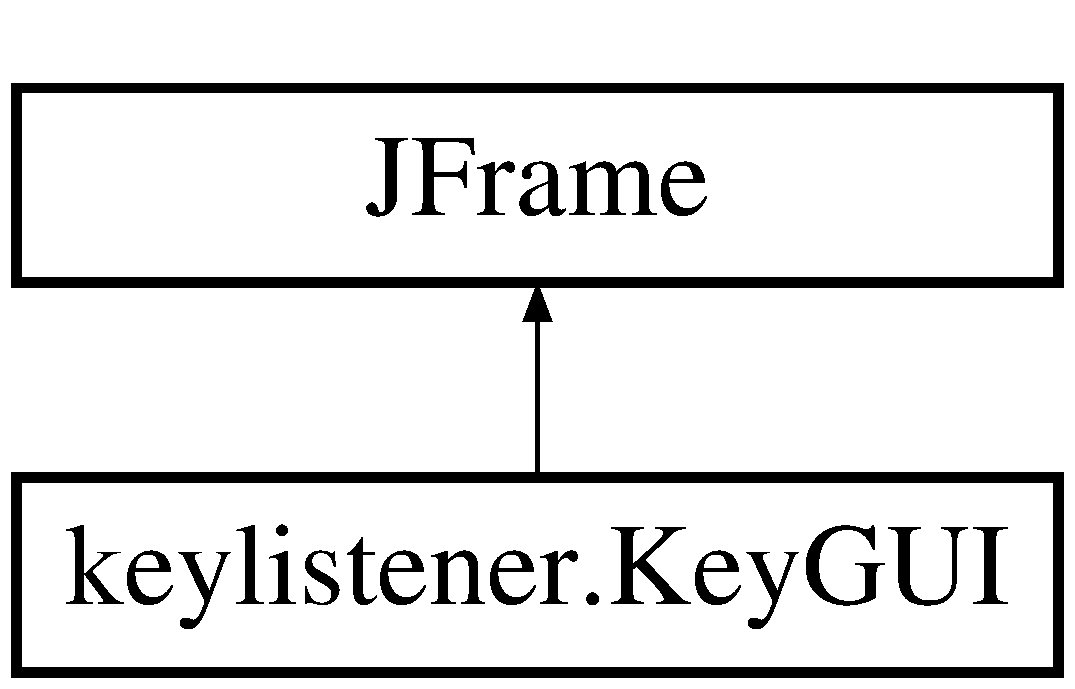
\includegraphics[height=2.000000cm]{classkeylistener_1_1_key_g_u_i}
\end{center}
\end{figure}
\subsection*{Classes}
\begin{DoxyCompactItemize}
\item 
class {\bfseries File\+Action}
\item 
class {\bfseries History\+Action}
\item 
class {\bfseries Search\+Action}
\end{DoxyCompactItemize}
\subsection*{Public Member Functions}
\begin{DoxyCompactItemize}
\item 
\hyperlink{classkeylistener_1_1_key_g_u_i_af48eff8474974c6c21eb0c36feaf65ad}{Key\+G\+UI} ()
\end{DoxyCompactItemize}
\subsection*{Static Public Member Functions}
\begin{DoxyCompactItemize}
\item 
static void \hyperlink{classkeylistener_1_1_key_g_u_i_ac0043858e116673e920af7f1542f5376}{main} (String args\mbox{[}$\,$\mbox{]})
\end{DoxyCompactItemize}
\subsection*{Private Member Functions}
\begin{DoxyCompactItemize}
\item 
void \hyperlink{classkeylistener_1_1_key_g_u_i_aee81c72d2c77342da78a38116883cf6f}{display\+History} ()
\item 
void \hyperlink{classkeylistener_1_1_key_g_u_i_a43be7b88fdba1420ee3f0d1c2c4c2748}{init\+Components} ()
\end{DoxyCompactItemize}
\subsection*{Private Attributes}
\begin{DoxyCompactItemize}
\item 
javax.\+swing.\+J\+Label \hyperlink{classkeylistener_1_1_key_g_u_i_ad2118979cc01e139f390529e68561b36}{lbl\+Date}
\item 
javax.\+swing.\+J\+Label \hyperlink{classkeylistener_1_1_key_g_u_i_a2d31eb97ae580ba4b09f1dd84a95bdb1}{lbl\+File\+Name}
\item 
javax.\+swing.\+J\+Label \hyperlink{classkeylistener_1_1_key_g_u_i_a330b92f9f544948e4e0b55307637ce6b}{lbl\+History\+File}
\item 
javax.\+swing.\+J\+Label \hyperlink{classkeylistener_1_1_key_g_u_i_aa0cbe65091b2645ad5f3e70be1d33702}{lbl\+History\+Search\+Keyword}
\item 
javax.\+swing.\+J\+Label \hyperlink{classkeylistener_1_1_key_g_u_i_a651562b55ac5b267be118fa85ee83b5d}{lbl\+Search}
\item 
javax.\+swing.\+J\+Label \hyperlink{classkeylistener_1_1_key_g_u_i_aa1b6d17eb8dab8ab033595be8cc66b81}{lbl\+Search\+Info}
\item 
javax.\+swing.\+J\+List$<$ String $>$ \hyperlink{classkeylistener_1_1_key_g_u_i_a53c4619456ef147805fdbd0f33527fa7}{list\+Result}
\item 
javax.\+swing.\+J\+Scroll\+Pane \hyperlink{classkeylistener_1_1_key_g_u_i_a036bb4e1e1c9b3761717272205313fe1}{scroll\+Pane}
\item 
javax.\+swing.\+J\+Text\+Field \hyperlink{classkeylistener_1_1_key_g_u_i_aa44762235ff4e3550950dded18266104}{txt\+Arrows}
\item 
javax.\+swing.\+J\+Text\+Field \hyperlink{classkeylistener_1_1_key_g_u_i_a49dc969b4b81645b57ce0ac461617031}{txt\+File\+Name}
\item 
javax.\+swing.\+J\+Text\+Field \hyperlink{classkeylistener_1_1_key_g_u_i_a12219fa977d21d4d00c2bdd827103a41}{txt\+Search}
\end{DoxyCompactItemize}


\subsection{Detailed Description}
\hyperlink{classkeylistener_1_1_key_g_u_i}{Key\+G\+UI} --- the main class that display G\+UI form to the user. \begin{DoxyAuthor}{Author}
Van Do 
\end{DoxyAuthor}
\begin{DoxyVersion}{Version}
1.\+0 
\end{DoxyVersion}


\subsection{Constructor \& Destructor Documentation}
\mbox{\Hypertarget{classkeylistener_1_1_key_g_u_i_af48eff8474974c6c21eb0c36feaf65ad}\label{classkeylistener_1_1_key_g_u_i_af48eff8474974c6c21eb0c36feaf65ad}} 
\index{keylistener\+::\+Key\+G\+UI@{keylistener\+::\+Key\+G\+UI}!Key\+G\+UI@{Key\+G\+UI}}
\index{Key\+G\+UI@{Key\+G\+UI}!keylistener\+::\+Key\+G\+UI@{keylistener\+::\+Key\+G\+UI}}
\subsubsection{\texorpdfstring{Key\+G\+U\+I()}{KeyGUI()}}
{\footnotesize\ttfamily keylistener.\+Key\+G\+U\+I.\+Key\+G\+UI (\begin{DoxyParamCaption}{ }\end{DoxyParamCaption})\hspace{0.3cm}{\ttfamily [inline]}}

Creates new form \hyperlink{classkeylistener_1_1_key_g_u_i}{Key\+G\+UI}. 

\subsection{Member Function Documentation}
\mbox{\Hypertarget{classkeylistener_1_1_key_g_u_i_aee81c72d2c77342da78a38116883cf6f}\label{classkeylistener_1_1_key_g_u_i_aee81c72d2c77342da78a38116883cf6f}} 
\index{keylistener\+::\+Key\+G\+UI@{keylistener\+::\+Key\+G\+UI}!display\+History@{display\+History}}
\index{display\+History@{display\+History}!keylistener\+::\+Key\+G\+UI@{keylistener\+::\+Key\+G\+UI}}
\subsubsection{\texorpdfstring{display\+History()}{displayHistory()}}
{\footnotesize\ttfamily void keylistener.\+Key\+G\+U\+I.\+display\+History (\begin{DoxyParamCaption}{ }\end{DoxyParamCaption})\hspace{0.3cm}{\ttfamily [inline]}, {\ttfamily [private]}}

Display the search item\textquotesingle{}s component from the front end. \mbox{\Hypertarget{classkeylistener_1_1_key_g_u_i_a43be7b88fdba1420ee3f0d1c2c4c2748}\label{classkeylistener_1_1_key_g_u_i_a43be7b88fdba1420ee3f0d1c2c4c2748}} 
\index{keylistener\+::\+Key\+G\+UI@{keylistener\+::\+Key\+G\+UI}!init\+Components@{init\+Components}}
\index{init\+Components@{init\+Components}!keylistener\+::\+Key\+G\+UI@{keylistener\+::\+Key\+G\+UI}}
\subsubsection{\texorpdfstring{init\+Components()}{initComponents()}}
{\footnotesize\ttfamily void keylistener.\+Key\+G\+U\+I.\+init\+Components (\begin{DoxyParamCaption}{ }\end{DoxyParamCaption})\hspace{0.3cm}{\ttfamily [inline]}, {\ttfamily [private]}}

This method is called from within the constructor to initialize the form. W\+A\+R\+N\+I\+NG\+: Do N\+OT modify this code. The content of this method is always regenerated by the Form Editor. \mbox{\Hypertarget{classkeylistener_1_1_key_g_u_i_ac0043858e116673e920af7f1542f5376}\label{classkeylistener_1_1_key_g_u_i_ac0043858e116673e920af7f1542f5376}} 
\index{keylistener\+::\+Key\+G\+UI@{keylistener\+::\+Key\+G\+UI}!main@{main}}
\index{main@{main}!keylistener\+::\+Key\+G\+UI@{keylistener\+::\+Key\+G\+UI}}
\subsubsection{\texorpdfstring{main()}{main()}}
{\footnotesize\ttfamily static void keylistener.\+Key\+G\+U\+I.\+main (\begin{DoxyParamCaption}\item[{String}]{args\mbox{[}$\,$\mbox{]} }\end{DoxyParamCaption})\hspace{0.3cm}{\ttfamily [inline]}, {\ttfamily [static]}}


\begin{DoxyParams}{Parameters}
{\em args} & the command line arguments \\
\hline
\end{DoxyParams}


\subsection{Member Data Documentation}
\mbox{\Hypertarget{classkeylistener_1_1_key_g_u_i_ad2118979cc01e139f390529e68561b36}\label{classkeylistener_1_1_key_g_u_i_ad2118979cc01e139f390529e68561b36}} 
\index{keylistener\+::\+Key\+G\+UI@{keylistener\+::\+Key\+G\+UI}!lbl\+Date@{lbl\+Date}}
\index{lbl\+Date@{lbl\+Date}!keylistener\+::\+Key\+G\+UI@{keylistener\+::\+Key\+G\+UI}}
\subsubsection{\texorpdfstring{lbl\+Date}{lblDate}}
{\footnotesize\ttfamily javax.\+swing.\+J\+Label keylistener.\+Key\+G\+U\+I.\+lbl\+Date\hspace{0.3cm}{\ttfamily [private]}}

\mbox{\Hypertarget{classkeylistener_1_1_key_g_u_i_a2d31eb97ae580ba4b09f1dd84a95bdb1}\label{classkeylistener_1_1_key_g_u_i_a2d31eb97ae580ba4b09f1dd84a95bdb1}} 
\index{keylistener\+::\+Key\+G\+UI@{keylistener\+::\+Key\+G\+UI}!lbl\+File\+Name@{lbl\+File\+Name}}
\index{lbl\+File\+Name@{lbl\+File\+Name}!keylistener\+::\+Key\+G\+UI@{keylistener\+::\+Key\+G\+UI}}
\subsubsection{\texorpdfstring{lbl\+File\+Name}{lblFileName}}
{\footnotesize\ttfamily javax.\+swing.\+J\+Label keylistener.\+Key\+G\+U\+I.\+lbl\+File\+Name\hspace{0.3cm}{\ttfamily [private]}}

\mbox{\Hypertarget{classkeylistener_1_1_key_g_u_i_a330b92f9f544948e4e0b55307637ce6b}\label{classkeylistener_1_1_key_g_u_i_a330b92f9f544948e4e0b55307637ce6b}} 
\index{keylistener\+::\+Key\+G\+UI@{keylistener\+::\+Key\+G\+UI}!lbl\+History\+File@{lbl\+History\+File}}
\index{lbl\+History\+File@{lbl\+History\+File}!keylistener\+::\+Key\+G\+UI@{keylistener\+::\+Key\+G\+UI}}
\subsubsection{\texorpdfstring{lbl\+History\+File}{lblHistoryFile}}
{\footnotesize\ttfamily javax.\+swing.\+J\+Label keylistener.\+Key\+G\+U\+I.\+lbl\+History\+File\hspace{0.3cm}{\ttfamily [private]}}

\mbox{\Hypertarget{classkeylistener_1_1_key_g_u_i_aa0cbe65091b2645ad5f3e70be1d33702}\label{classkeylistener_1_1_key_g_u_i_aa0cbe65091b2645ad5f3e70be1d33702}} 
\index{keylistener\+::\+Key\+G\+UI@{keylistener\+::\+Key\+G\+UI}!lbl\+History\+Search\+Keyword@{lbl\+History\+Search\+Keyword}}
\index{lbl\+History\+Search\+Keyword@{lbl\+History\+Search\+Keyword}!keylistener\+::\+Key\+G\+UI@{keylistener\+::\+Key\+G\+UI}}
\subsubsection{\texorpdfstring{lbl\+History\+Search\+Keyword}{lblHistorySearchKeyword}}
{\footnotesize\ttfamily javax.\+swing.\+J\+Label keylistener.\+Key\+G\+U\+I.\+lbl\+History\+Search\+Keyword\hspace{0.3cm}{\ttfamily [private]}}

\mbox{\Hypertarget{classkeylistener_1_1_key_g_u_i_a651562b55ac5b267be118fa85ee83b5d}\label{classkeylistener_1_1_key_g_u_i_a651562b55ac5b267be118fa85ee83b5d}} 
\index{keylistener\+::\+Key\+G\+UI@{keylistener\+::\+Key\+G\+UI}!lbl\+Search@{lbl\+Search}}
\index{lbl\+Search@{lbl\+Search}!keylistener\+::\+Key\+G\+UI@{keylistener\+::\+Key\+G\+UI}}
\subsubsection{\texorpdfstring{lbl\+Search}{lblSearch}}
{\footnotesize\ttfamily javax.\+swing.\+J\+Label keylistener.\+Key\+G\+U\+I.\+lbl\+Search\hspace{0.3cm}{\ttfamily [private]}}

\mbox{\Hypertarget{classkeylistener_1_1_key_g_u_i_aa1b6d17eb8dab8ab033595be8cc66b81}\label{classkeylistener_1_1_key_g_u_i_aa1b6d17eb8dab8ab033595be8cc66b81}} 
\index{keylistener\+::\+Key\+G\+UI@{keylistener\+::\+Key\+G\+UI}!lbl\+Search\+Info@{lbl\+Search\+Info}}
\index{lbl\+Search\+Info@{lbl\+Search\+Info}!keylistener\+::\+Key\+G\+UI@{keylistener\+::\+Key\+G\+UI}}
\subsubsection{\texorpdfstring{lbl\+Search\+Info}{lblSearchInfo}}
{\footnotesize\ttfamily javax.\+swing.\+J\+Label keylistener.\+Key\+G\+U\+I.\+lbl\+Search\+Info\hspace{0.3cm}{\ttfamily [private]}}

\mbox{\Hypertarget{classkeylistener_1_1_key_g_u_i_a53c4619456ef147805fdbd0f33527fa7}\label{classkeylistener_1_1_key_g_u_i_a53c4619456ef147805fdbd0f33527fa7}} 
\index{keylistener\+::\+Key\+G\+UI@{keylistener\+::\+Key\+G\+UI}!list\+Result@{list\+Result}}
\index{list\+Result@{list\+Result}!keylistener\+::\+Key\+G\+UI@{keylistener\+::\+Key\+G\+UI}}
\subsubsection{\texorpdfstring{list\+Result}{listResult}}
{\footnotesize\ttfamily javax.\+swing.\+J\+List$<$String$>$ keylistener.\+Key\+G\+U\+I.\+list\+Result\hspace{0.3cm}{\ttfamily [private]}}

\mbox{\Hypertarget{classkeylistener_1_1_key_g_u_i_a036bb4e1e1c9b3761717272205313fe1}\label{classkeylistener_1_1_key_g_u_i_a036bb4e1e1c9b3761717272205313fe1}} 
\index{keylistener\+::\+Key\+G\+UI@{keylistener\+::\+Key\+G\+UI}!scroll\+Pane@{scroll\+Pane}}
\index{scroll\+Pane@{scroll\+Pane}!keylistener\+::\+Key\+G\+UI@{keylistener\+::\+Key\+G\+UI}}
\subsubsection{\texorpdfstring{scroll\+Pane}{scrollPane}}
{\footnotesize\ttfamily javax.\+swing.\+J\+Scroll\+Pane keylistener.\+Key\+G\+U\+I.\+scroll\+Pane\hspace{0.3cm}{\ttfamily [private]}}

\mbox{\Hypertarget{classkeylistener_1_1_key_g_u_i_aa44762235ff4e3550950dded18266104}\label{classkeylistener_1_1_key_g_u_i_aa44762235ff4e3550950dded18266104}} 
\index{keylistener\+::\+Key\+G\+UI@{keylistener\+::\+Key\+G\+UI}!txt\+Arrows@{txt\+Arrows}}
\index{txt\+Arrows@{txt\+Arrows}!keylistener\+::\+Key\+G\+UI@{keylistener\+::\+Key\+G\+UI}}
\subsubsection{\texorpdfstring{txt\+Arrows}{txtArrows}}
{\footnotesize\ttfamily javax.\+swing.\+J\+Text\+Field keylistener.\+Key\+G\+U\+I.\+txt\+Arrows\hspace{0.3cm}{\ttfamily [private]}}

\mbox{\Hypertarget{classkeylistener_1_1_key_g_u_i_a49dc969b4b81645b57ce0ac461617031}\label{classkeylistener_1_1_key_g_u_i_a49dc969b4b81645b57ce0ac461617031}} 
\index{keylistener\+::\+Key\+G\+UI@{keylistener\+::\+Key\+G\+UI}!txt\+File\+Name@{txt\+File\+Name}}
\index{txt\+File\+Name@{txt\+File\+Name}!keylistener\+::\+Key\+G\+UI@{keylistener\+::\+Key\+G\+UI}}
\subsubsection{\texorpdfstring{txt\+File\+Name}{txtFileName}}
{\footnotesize\ttfamily javax.\+swing.\+J\+Text\+Field keylistener.\+Key\+G\+U\+I.\+txt\+File\+Name\hspace{0.3cm}{\ttfamily [private]}}

\mbox{\Hypertarget{classkeylistener_1_1_key_g_u_i_a12219fa977d21d4d00c2bdd827103a41}\label{classkeylistener_1_1_key_g_u_i_a12219fa977d21d4d00c2bdd827103a41}} 
\index{keylistener\+::\+Key\+G\+UI@{keylistener\+::\+Key\+G\+UI}!txt\+Search@{txt\+Search}}
\index{txt\+Search@{txt\+Search}!keylistener\+::\+Key\+G\+UI@{keylistener\+::\+Key\+G\+UI}}
\subsubsection{\texorpdfstring{txt\+Search}{txtSearch}}
{\footnotesize\ttfamily javax.\+swing.\+J\+Text\+Field keylistener.\+Key\+G\+U\+I.\+txt\+Search\hspace{0.3cm}{\ttfamily [private]}}



The documentation for this class was generated from the following file\+:\begin{DoxyCompactItemize}
\item 
src/keylistener/\hyperlink{_key_g_u_i_8java}{Key\+G\+U\+I.\+java}\end{DoxyCompactItemize}

\hypertarget{classkeylistener_1_1_read_file}{}\section{keylistener.\+Read\+File Class Reference}
\label{classkeylistener_1_1_read_file}\index{keylistener.\+Read\+File@{keylistener.\+Read\+File}}
\subsection*{Public Member Functions}
\begin{DoxyCompactItemize}
\item 
Boolean \hyperlink{classkeylistener_1_1_read_file_a2438c71e757495e44c2892ff821ad189}{is\+File} (String file\+Name)
\item 
List$<$ String $>$ \hyperlink{classkeylistener_1_1_read_file_a889398266aa6c457b948b5ab40a2548e}{read\+File} (String file\+Name)
\end{DoxyCompactItemize}
\subsection*{Private Attributes}
\begin{DoxyCompactItemize}
\item 
Buffered\+Reader \hyperlink{classkeylistener_1_1_read_file_a18760d47084093fc16d97fc105c48c1e}{reader}
\end{DoxyCompactItemize}


\subsection{Detailed Description}
\hyperlink{classkeylistener_1_1_read_file}{Read\+File} --- this class allows to check the existence of the file and read file. \begin{DoxyAuthor}{Author}
Van Do 
\end{DoxyAuthor}


\subsection{Member Function Documentation}
\mbox{\Hypertarget{classkeylistener_1_1_read_file_a2438c71e757495e44c2892ff821ad189}\label{classkeylistener_1_1_read_file_a2438c71e757495e44c2892ff821ad189}} 
\index{keylistener\+::\+Read\+File@{keylistener\+::\+Read\+File}!is\+File@{is\+File}}
\index{is\+File@{is\+File}!keylistener\+::\+Read\+File@{keylistener\+::\+Read\+File}}
\subsubsection{\texorpdfstring{is\+File()}{isFile()}}
{\footnotesize\ttfamily Boolean keylistener.\+Read\+File.\+is\+File (\begin{DoxyParamCaption}\item[{String}]{file\+Name }\end{DoxyParamCaption})\hspace{0.3cm}{\ttfamily [inline]}}

Check if file does exist. 
\begin{DoxyParams}{Parameters}
{\em file\+Name} & -\/ the name of the file. \\
\hline
\end{DoxyParams}
\begin{DoxyReturn}{Returns}
if the file is exists or not. 
\end{DoxyReturn}
\mbox{\Hypertarget{classkeylistener_1_1_read_file_a889398266aa6c457b948b5ab40a2548e}\label{classkeylistener_1_1_read_file_a889398266aa6c457b948b5ab40a2548e}} 
\index{keylistener\+::\+Read\+File@{keylistener\+::\+Read\+File}!read\+File@{read\+File}}
\index{read\+File@{read\+File}!keylistener\+::\+Read\+File@{keylistener\+::\+Read\+File}}
\subsubsection{\texorpdfstring{read\+File()}{readFile()}}
{\footnotesize\ttfamily List$<$String$>$ keylistener.\+Read\+File.\+read\+File (\begin{DoxyParamCaption}\item[{String}]{file\+Name }\end{DoxyParamCaption})\hspace{0.3cm}{\ttfamily [inline]}}

Read all lines from the file and store into list. 
\begin{DoxyParams}{Parameters}
{\em file\+Name} & -\/ the name of the file. \\
\hline
\end{DoxyParams}
\begin{DoxyReturn}{Returns}
the list of lines from the file. 
\end{DoxyReturn}

\begin{DoxyExceptions}{Exceptions}
{\em File\+Not\+Found\+Exception} & -\/ catch errors if file does not exists. \\
\hline
{\em I\+O\+Exception} & -\/ catch errors if lines have incorrect variable declaration. \\
\hline
\end{DoxyExceptions}


\subsection{Member Data Documentation}
\mbox{\Hypertarget{classkeylistener_1_1_read_file_a18760d47084093fc16d97fc105c48c1e}\label{classkeylistener_1_1_read_file_a18760d47084093fc16d97fc105c48c1e}} 
\index{keylistener\+::\+Read\+File@{keylistener\+::\+Read\+File}!reader@{reader}}
\index{reader@{reader}!keylistener\+::\+Read\+File@{keylistener\+::\+Read\+File}}
\subsubsection{\texorpdfstring{reader}{reader}}
{\footnotesize\ttfamily Buffered\+Reader keylistener.\+Read\+File.\+reader\hspace{0.3cm}{\ttfamily [private]}}

Read lines from any file 

The documentation for this class was generated from the following file\+:\begin{DoxyCompactItemize}
\item 
src/keylistener/\hyperlink{_read_file_8java}{Read\+File.\+java}\end{DoxyCompactItemize}

\hypertarget{classkeylistener_1_1_search}{}\section{keylistener.\+Search Class Reference}
\label{classkeylistener_1_1_search}\index{keylistener.\+Search@{keylistener.\+Search}}
\subsection*{Public Member Functions}
\begin{DoxyCompactItemize}
\item 
List$<$ String $>$ \hyperlink{classkeylistener_1_1_search_aca84b495ee4365467104d2431d2fd974}{search\+List} (String keyword, String\mbox{[}$\,$\mbox{]} list)
\end{DoxyCompactItemize}


\subsection{Detailed Description}
\hyperlink{classkeylistener_1_1_search}{Search} --- this class will use a linear search method to compare each line that contains the keyword. \begin{DoxyAuthor}{Author}
Van Do 
\end{DoxyAuthor}


\subsection{Member Function Documentation}
\mbox{\Hypertarget{classkeylistener_1_1_search_aca84b495ee4365467104d2431d2fd974}\label{classkeylistener_1_1_search_aca84b495ee4365467104d2431d2fd974}} 
\index{keylistener\+::\+Search@{keylistener\+::\+Search}!search\+List@{search\+List}}
\index{search\+List@{search\+List}!keylistener\+::\+Search@{keylistener\+::\+Search}}
\subsubsection{\texorpdfstring{search\+List()}{searchList()}}
{\footnotesize\ttfamily List$<$String$>$ keylistener.\+Search.\+search\+List (\begin{DoxyParamCaption}\item[{String}]{keyword,  }\item[{String \mbox{[}$\,$\mbox{]}}]{list }\end{DoxyParamCaption})\hspace{0.3cm}{\ttfamily [inline]}}

\hyperlink{classkeylistener_1_1_search}{Search} through the line from the file and return the list of results that contain keyword. 
\begin{DoxyParams}{Parameters}
{\em keyword} & -\/ the input that the user wants to search for each line. \\
\hline
{\em list} & -\/ all of the lines from the file. \\
\hline
\end{DoxyParams}
\begin{DoxyReturn}{Returns}
the list of compared line that contains the keyword. 
\end{DoxyReturn}


The documentation for this class was generated from the following file\+:\begin{DoxyCompactItemize}
\item 
src/keylistener/\hyperlink{_search_8java}{Search.\+java}\end{DoxyCompactItemize}

\chapter{File Documentation}
\hypertarget{_file_history_8java}{}\section{src/keylistener/\+File\+History.java File Reference}
\label{_file_history_8java}\index{src/keylistener/\+File\+History.\+java@{src/keylistener/\+File\+History.\+java}}
\subsection*{Classes}
\begin{DoxyCompactItemize}
\item 
class \hyperlink{classkeylistener_1_1_file_history}{keylistener.\+File\+History}
\end{DoxyCompactItemize}
\subsection*{Packages}
\begin{DoxyCompactItemize}
\item 
package \hyperlink{namespacekeylistener}{keylistener}
\end{DoxyCompactItemize}

\hypertarget{_key_g_u_i_8java}{}\section{src/keylistener/\+Key\+G\+UI.java File Reference}
\label{_key_g_u_i_8java}\index{src/keylistener/\+Key\+G\+U\+I.\+java@{src/keylistener/\+Key\+G\+U\+I.\+java}}
\subsection*{Classes}
\begin{DoxyCompactItemize}
\item 
class \hyperlink{classkeylistener_1_1_key_g_u_i}{keylistener.\+Key\+G\+UI}
\item 
class {\bfseries keylistener.\+Key\+G\+U\+I.\+File\+Action}
\item 
class {\bfseries keylistener.\+Key\+G\+U\+I.\+Search\+Action}
\item 
class {\bfseries keylistener.\+Key\+G\+U\+I.\+History\+Action}
\end{DoxyCompactItemize}
\subsection*{Packages}
\begin{DoxyCompactItemize}
\item 
package \hyperlink{namespacekeylistener}{keylistener}
\end{DoxyCompactItemize}

\hypertarget{_read_file_8java}{}\section{src/keylistener/\+Read\+File.java File Reference}
\label{_read_file_8java}\index{src/keylistener/\+Read\+File.\+java@{src/keylistener/\+Read\+File.\+java}}
\subsection*{Classes}
\begin{DoxyCompactItemize}
\item 
class \hyperlink{classkeylistener_1_1_read_file}{keylistener.\+Read\+File}
\end{DoxyCompactItemize}
\subsection*{Packages}
\begin{DoxyCompactItemize}
\item 
package \hyperlink{namespacekeylistener}{keylistener}
\end{DoxyCompactItemize}

\hypertarget{_search_8java}{}\section{src/keylistener/\+Search.java File Reference}
\label{_search_8java}\index{src/keylistener/\+Search.\+java@{src/keylistener/\+Search.\+java}}
\subsection*{Classes}
\begin{DoxyCompactItemize}
\item 
class \hyperlink{classkeylistener_1_1_search}{keylistener.\+Search}
\end{DoxyCompactItemize}
\subsection*{Packages}
\begin{DoxyCompactItemize}
\item 
package \hyperlink{namespacekeylistener}{keylistener}
\end{DoxyCompactItemize}

%--- End generated contents ---

% Index
\backmatter
\newpage
\phantomsection
\clearemptydoublepage
\addcontentsline{toc}{chapter}{Index}
\printindex

\end{document}
